\section{Results}
\begin{figure*}[t]
\centering
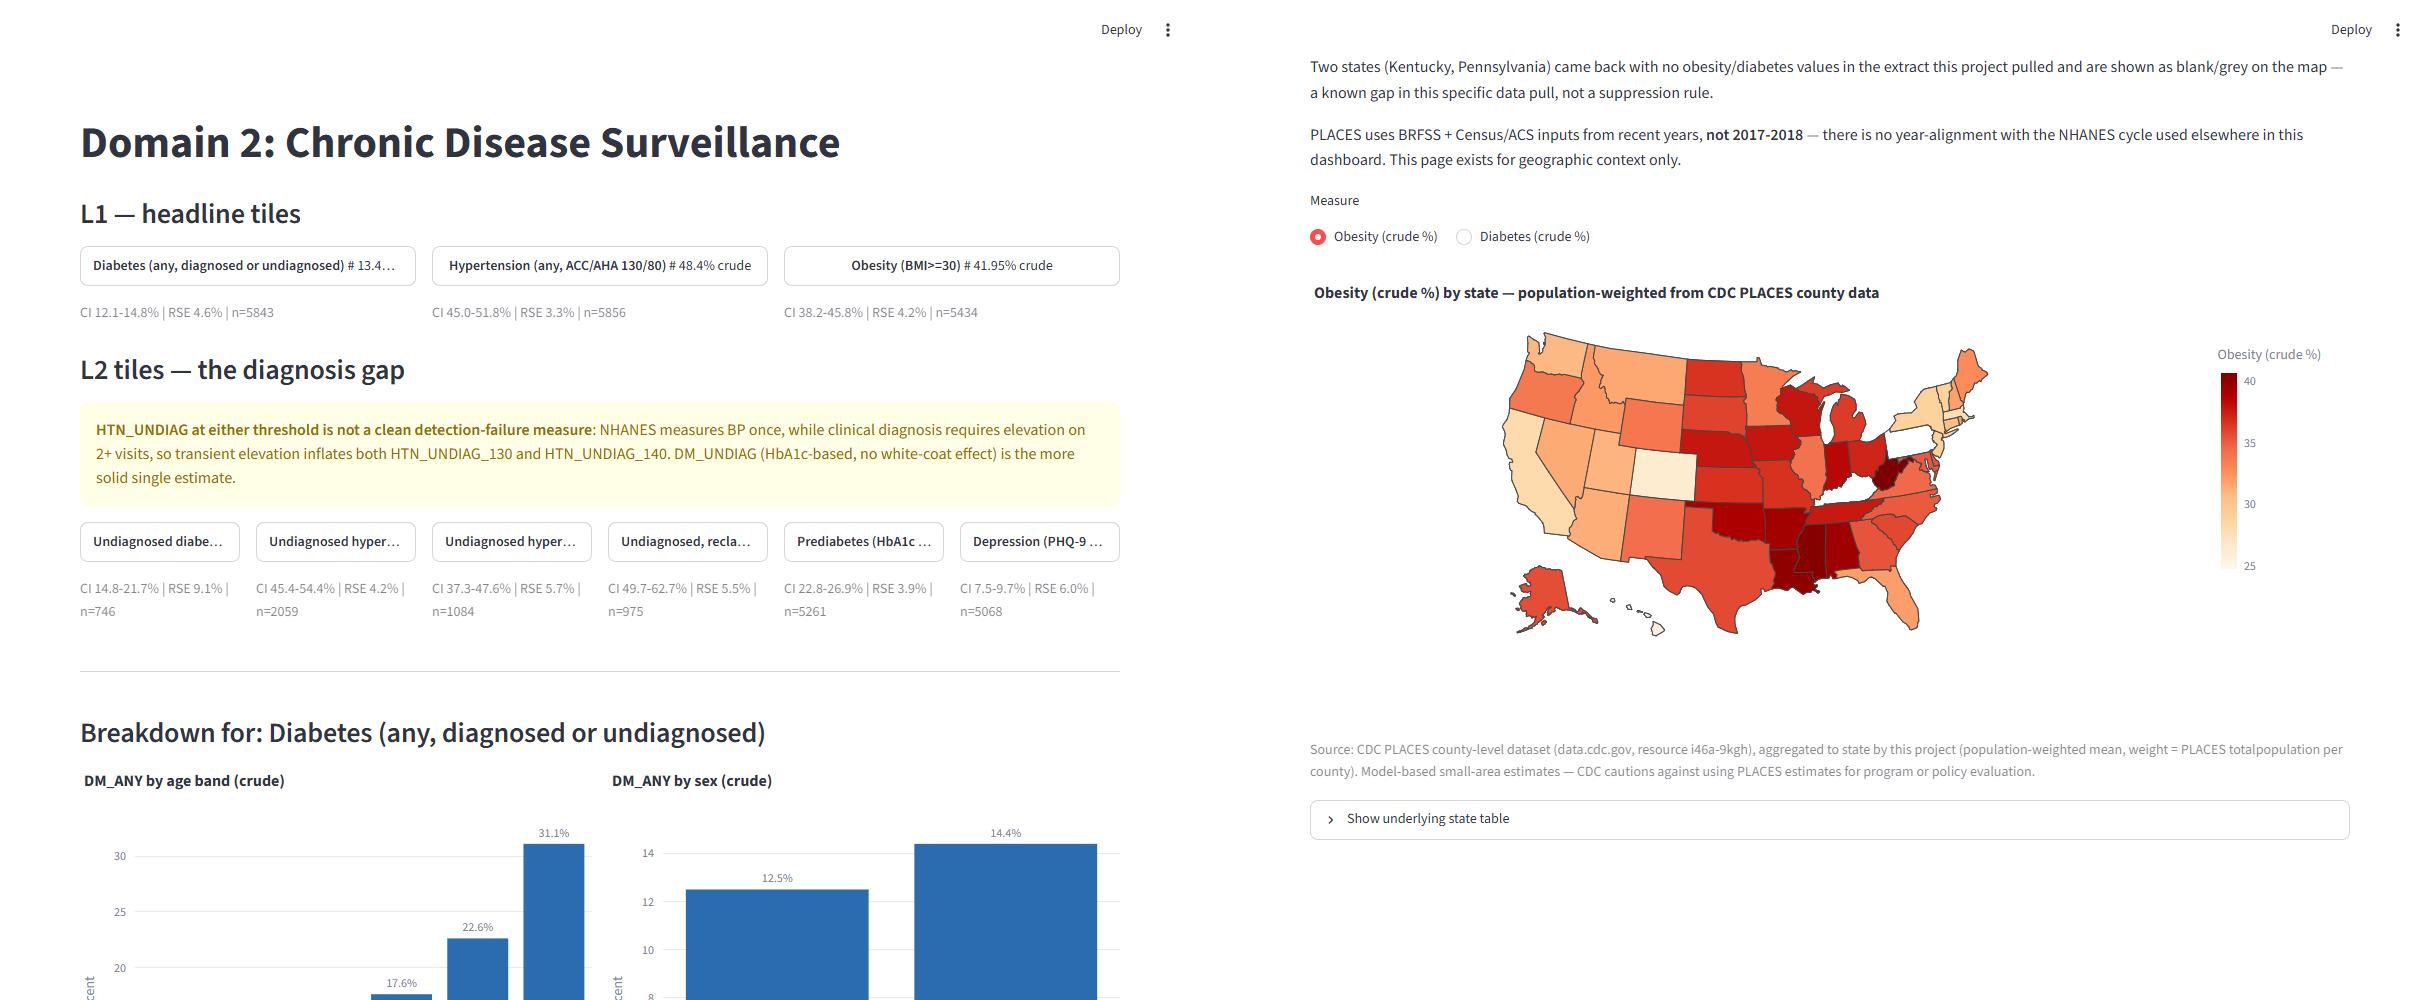
\includegraphics[width=0.64\textwidth]{figures/dashboard_pair.png}
\caption{Streamlit dashboard. Left: chronic-disease page with Level~1 headline tiles, the diagnosis-gap tiles and Level~2 breakdowns. Right: CDC PLACES state choropleth (obesity, population-weighted county estimates), labelled as a separate model-based source. Source: NHANES 2017--2018, \texttt{out/kpi\_long.csv}.}
\label{fig:dash}
\end{figure*}

\begin{figure*}[t]
\centering
\begin{minipage}{0.48\textwidth}\centering
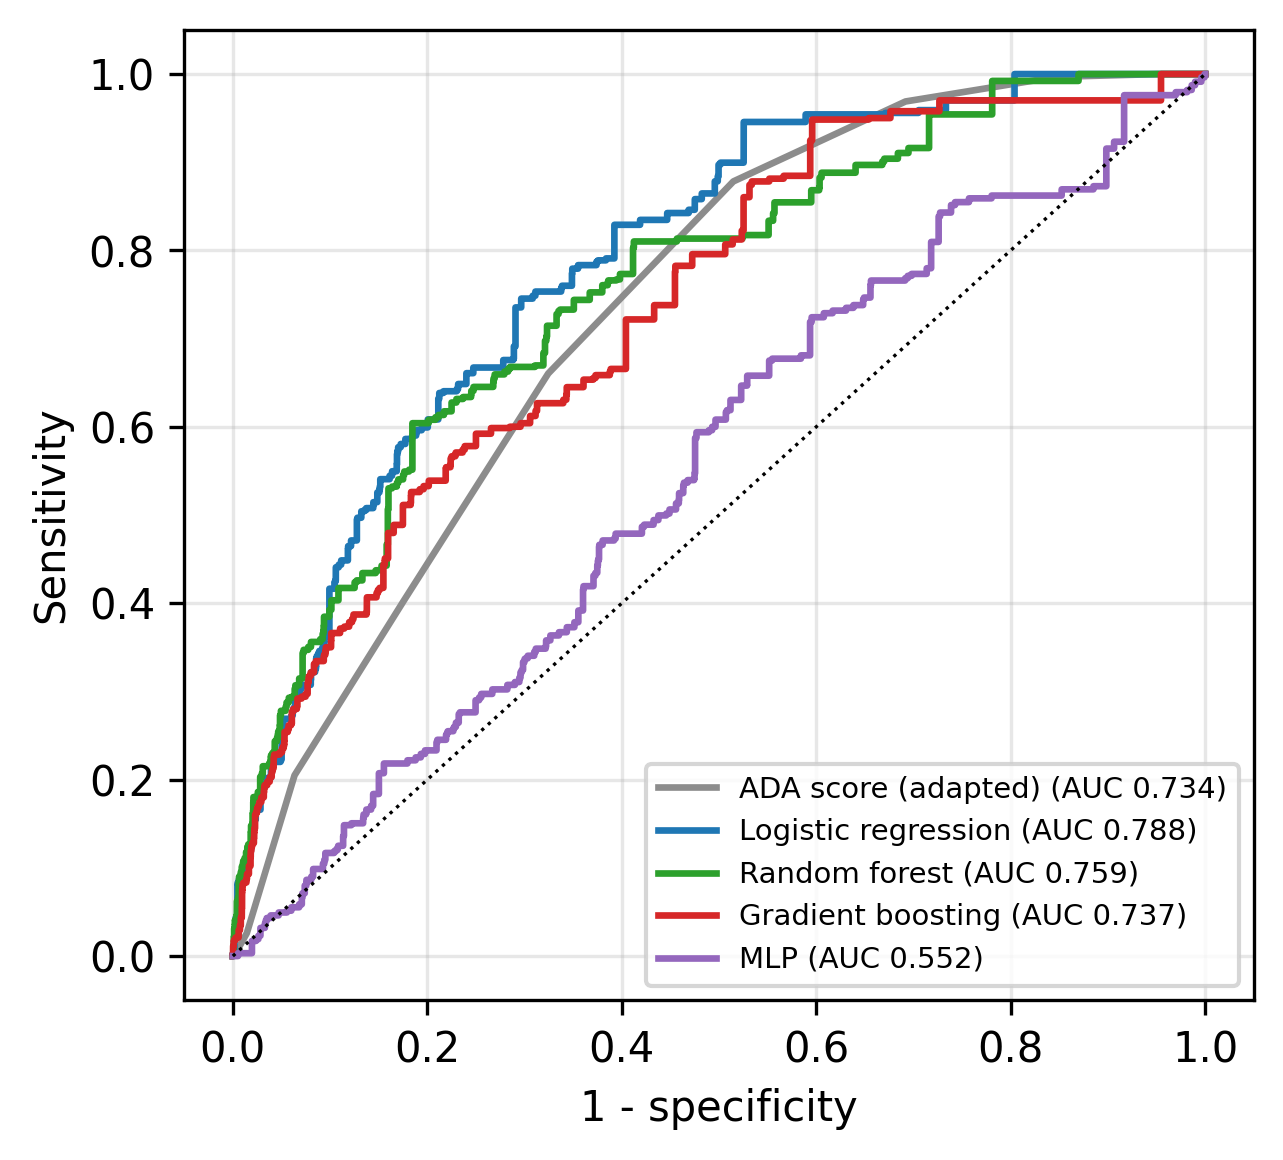
\includegraphics[width=0.72\linewidth]{figures/ml_roc.png}\\
\footnotesize (a) Weighted ROC curves, pooled out-of-fold predictions
\end{minipage}\hfill
\begin{minipage}{0.48\textwidth}\centering
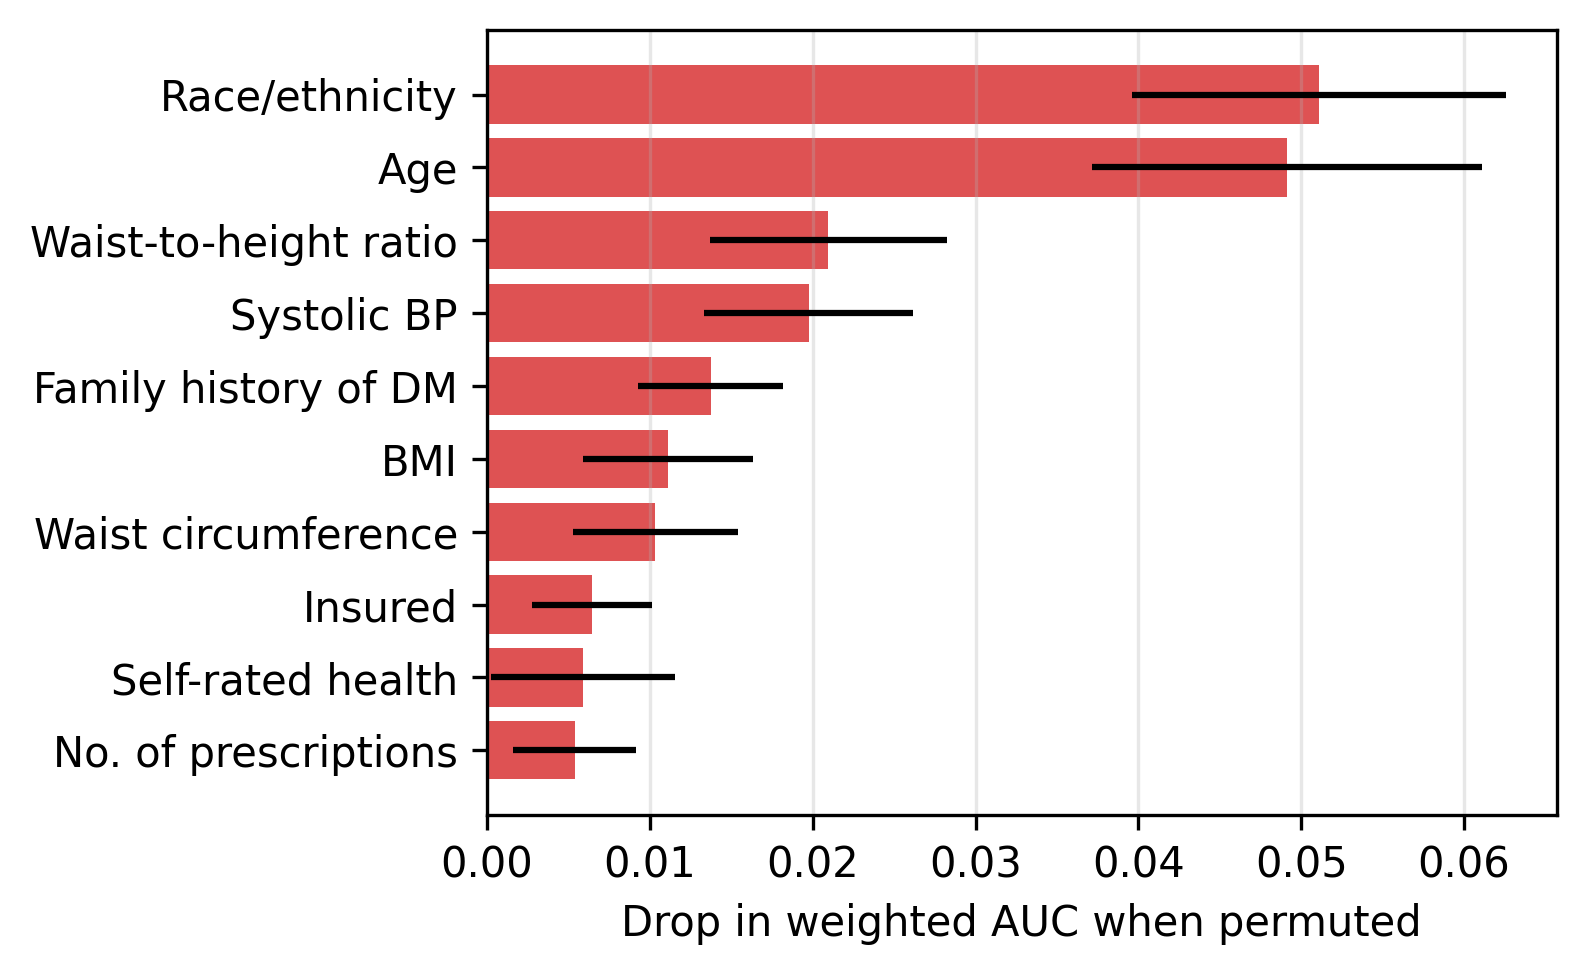
\includegraphics[width=0.86\linewidth]{figures/ml_importance.png}\\
\footnotesize (b) Permutation importance, final logistic regression
\end{minipage}
\caption{Screening results (NHANES 2017--2018, adults 20+ never told they had diabetes, MEC weights, $n=4{,}051$). Importance is the mean $\pm$ SD drop in weighted AUC over 10 permutations.}
\label{fig:roc}
\end{figure*}

\subsection{KPI estimates and the diagnosis gap}
Table~\ref{tab:kpi} gives the headline estimates. Of the 612 cells, 53 (8.7\%) were suppressed. Among adults whose HbA1c was 6.5\% or higher, an estimated 18.0\% (95\% CI 14.8--21.7, $n=746$) had never been told they had diabetes. They represent about 23.5 million adults, so roughly 4.2 million had undiagnosed diabetes. Treating ``borderline'' answers as undiagnosed gives 23.4\% (19.5--27.7), close to the 23.3\% of Wang \textit{et al.} \cite{wang2021}. Undiagnosed hypertension was 49.9\% at 130/80 and 42.4\% at 140/90, on different denominators. Both are far above the roughly 23\% unawareness of Muntner \textit{et al.} \cite{muntner2020}, because our denominator excludes treated, controlled hypertensives and blood pressure was measured at one visit. HbA1c has neither problem, so diabetes anchors the diagnosis-gap finding.

\begin{table}[t]
\caption{Headline KPI Estimates, Adults 18+, NHANES 2017--2018}
\label{tab:kpi}
\centering
\footnotesize
\setlength{\tabcolsep}{3pt}
\begin{tabular}{@{}lrrrr@{}}
\toprule
\textbf{Indicator} & \textbf{\%} & \textbf{95\% CI} & \textbf{RSE} & \textbf{$n$} \\
\midrule
\multicolumn{5}{@{}l}{\textit{Chronic disease}} \\
Any diabetes & 13.4 & 12.1--14.8 & 4.6 & 5,843 \\
Undiagnosed diabetes$^a$ & 18.0 & 14.8--21.7 & 9.1 & 746 \\
Prediabetes (HbA1c 5.7--6.4\%) & 24.8 & 22.8--26.9 & 3.9 & 5,261 \\
Hypertension (130/80 or told) & 48.4 & 45.0--51.8 & 3.3 & 5,856 \\
Undiagnosed HTN, 130/80$^a$ & 49.9 & 45.4--54.4 & 4.2 & 2,059 \\
Undiagnosed HTN, 140/90$^a$ & 42.4 & 37.3--47.6 & 5.7 & 1,084 \\
Obesity (BMI $\geq$30) & 42.0 & 38.2--45.8 & 4.2 & 5,434 \\
Depression (PHQ-9 $\geq$10) & 8.6 & 7.5--9.7 & 6.0 & 5,068 \\
\multicolumn{5}{@{}l}{\textit{Utilisation and experience}} \\
Fair/poor self-rated health & 18.6 & 16.6--20.8 & 5.3 & 5,849 \\
Admitted, past 12 months & 11.0 & 10.1--11.9 & 4.0 & 5,854 \\
$\geq$4 care contacts & 20.7 & 19.4--22.0 & 2.9 & 5,842 \\
\multicolumn{5}{@{}l}{\textit{Access}} \\
Uninsured & 13.9 & 10.3--18.5 & 13.7 & 5,837 \\
Has usual source of care & 81.2 & 78.3--83.8 & 1.6 & 5,817 \\
Polypharmacy ($\geq$5 Rx) & 16.5 & 14.5--18.7 & 6.0 & 5,856 \\
\bottomrule
\multicolumn{5}{@{}l}{\scriptsize $^a$Denominator: adults above the laboratory or measured threshold.}\\
\multicolumn{5}{@{}l}{\scriptsize Logit intervals with $t_{0.975,15}$; RSE in \%.}
\end{tabular}
\end{table}

\subsection{Income inequality}
Access and self-reported outcomes were strongly concentrated among poorer adults: uninsured $C=-0.424$ (Erreygers $E=-0.236$), fair or poor health $-0.270$ ($E=-0.201$) and depression $-0.257$ ($E=-0.088$), while undiagnosed diabetes was almost flat ($C=-0.011$) and undiagnosed hypertension was slightly concentrated among richer adults ($+0.029$ and $+0.052$). Within age bands the uninsured gradient was steeper ($-0.39$ to $-0.53$ at 30--69), so Medicare above 65 does not explain it. For any diabetes the pooled index ($-0.011$) hid a stronger gradient at 60--69 ($-0.127$), because poorer respondents are younger. Undiagnosed diabetes stayed flat in the only well-populated band ($-0.002$ at 60--69): insurance would narrow the access gap, but screening has to reach all income groups.



\subsection{Validation against published estimates}
Age-standardised obesity (41.8\%) was within one point of Hales \textit{et al.} (42.4\%, ages 20+) \cite{hales2020}. Hypertension (45.0\%) matched Ostchega \textit{et al.} (45.4\%) \cite{ostchega2020}, but their definition also counts medication users, so the match may hide offsetting differences. Any diabetes (13.5\%) was close to the national 13.2\% (12.0--14.5) \cite{cdc_ndsr} even though ours omits fasting glucose, an open question. Undiagnosed diabetes could not be standardised, as only four of eight age groups were estimable.
